\documentclass[tikz,border=6pt]{standalone}
\usetikzlibrary{arrows.meta,positioning}
\begin{document}
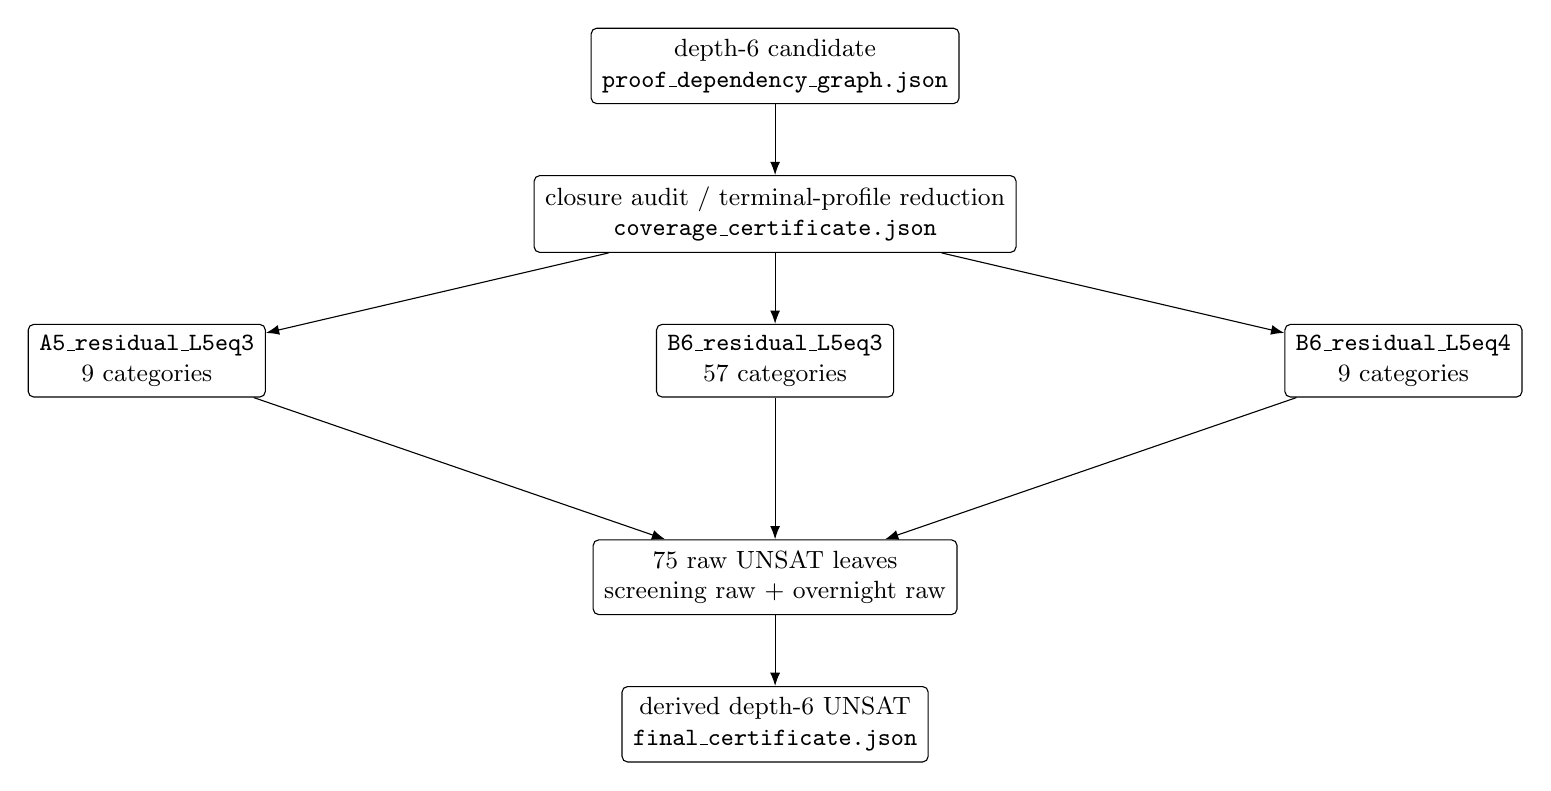
\begin{tikzpicture}[
  node distance=9mm and 12mm,
  box/.style={draw, rounded corners=2pt, align=center, font=\small, inner sep=4pt},
  edge/.style={-Latex}
]
\node[box] (candidate) {depth-6 candidate\\\texttt{proof\_dependency\_graph.json}};
\node[box, below=of candidate] (closure) {closure audit / terminal-profile reduction\\\texttt{coverage\_certificate.json}};
\node[box, below left=of closure, xshift=-22mm] (a5) {\texttt{A5\_residual\_L5eq3}\\9 categories};
\node[box, below=of closure] (b63) {\texttt{B6\_residual\_L5eq3}\\57 categories};
\node[box, below right=of closure, xshift=22mm] (b64) {\texttt{B6\_residual\_L5eq4}\\9 categories};
\node[box, below=18mm of b63] (leaves) {75 raw UNSAT leaves\\screening raw + overnight raw};
\node[box, below=of leaves] (unsat) {derived depth-6 UNSAT\\\texttt{final\_certificate.json}};
\draw[edge] (candidate) -- (closure);
\draw[edge] (closure) -- (a5);
\draw[edge] (closure) -- (b63);
\draw[edge] (closure) -- (b64);
\draw[edge] (a5) -- (leaves);
\draw[edge] (b63) -- (leaves);
\draw[edge] (b64) -- (leaves);
\draw[edge] (leaves) -- (unsat);
\end{tikzpicture}
\end{document}
